\chapter{Problem Statement}
\label{ch:problem_statement}

\section{Formal Problem Formulation}
\label{sec:problem_formulation}
Formally, let a citizen user $U$ interact with the public socio-legal domain through a natural language query $Q = \{w_1, w_2, \dots, w_n\}$ or an uploaded legal document $D_{in} \in \{\text{PDF, Image}\}$. The citizen's objective is to obtain an actionable, legally accurate, and plain-language guidance response $R$, accompanied by a set of verifiable statutory citations $C = \{c_1, c_2, \dots, c_k\}$, a set of qualifying government welfare schemes $S = \{s_1, s_2, \dots, s_m\}$, and an extracted document structured evidence record $E_{doc}$.

The multi-domain civic intelligence challenge can be modeled as finding an optimal mapping function $\Phi$:
\begin{equation}
\Phi: (Q, D_{in}, \mathcal{K}_{statute}, \mathcal{K}_{scheme}, \mathcal{G}_{civic}) \longrightarrow (R, C, S, E_{doc}, \mathcal{A}_{next})
\label{eq:mapping_func}
\end{equation}
subject to the following hard constraints:
\begin{enumerate}
    \item \textbf{Citation Verifiability Constraint:} $\forall c_i \in C$, $c_i$ must map directly to an authoritative statutory section in $\mathcal{K}_{statute}$ with empirical text grounding $\text{Sim}(c_i, \mathcal{K}_{statute}) \ge \tau_{threshold}$. No fabricated or hallucinated citations are permitted.
    \item \textbf{Temporal Freshness Constraint:} $\forall c_i \in C$, the statutory provision must be legally in force at timestamp $t_{query}$ (i.e., repealed provisions such as IPC sections must be mapped to their corresponding BNS 2023 equivalents).
    \item \textbf{Data Privacy and Confidentiality Constraint:} The storage of $D_{in}$ and processing of $Q$ must strictly comply with the Digital Personal Data Protection Act 2023, ensuring zero unauthorized cross-tenant data access, isolated private object storage, and immediate cascade deletion upon user request:
    \begin{equation}
    \text{Purge}(U) \Longrightarrow \forall d \in D_U, \quad \text{S3Delete}(d) \land \text{DBDelete}(d) = \text{True}
    \end{equation}
    \item \textbf{Sub-Second Computational Latency:} The triage of $Q$ and heuristic extraction of $D_{in}$ must execute within latency $\le 2.0$ seconds on serverless cloud compute infrastructure.
\end{enumerate}

\section{Logical Connection: From Problem to Solution}
\label{sec:logical_connection}
The logical progression from the identified civic failure modes to our architectural design is visualized in Figure~\ref{fig:problem_to_solution_flow}.

\begin{figure}[H]
\centering
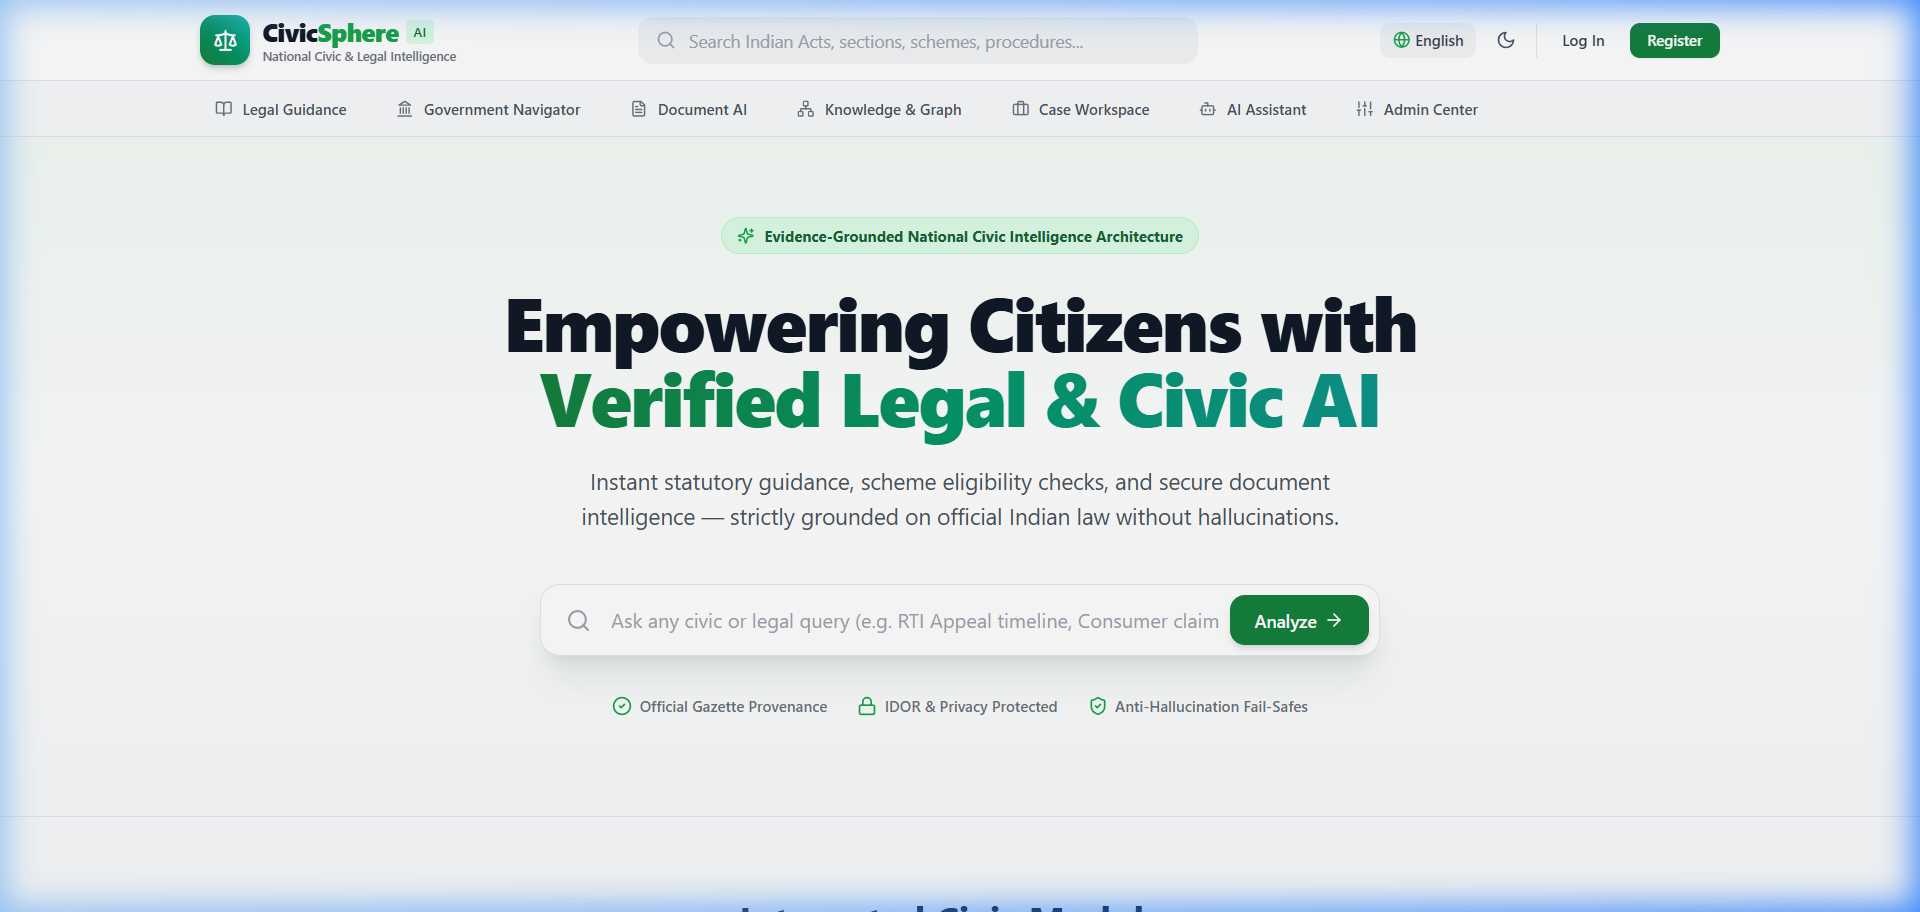
\includegraphics[width=0.9\textwidth]{images/homepage_view.png}
\caption{Logical progression from citizen problem to evidence-grounded civic guidance.}
\label{fig:problem_to_solution_flow}
\end{figure}

The transition operates across three sequential computational layers:
\begin{itemize}
    \item \textbf{Input Disambiguation Layer:} Translates ambiguous, emotionally distressed natural language queries into normalized legal entities, statutory domains, and administrative locations.
    \item \textbf{Hybrid Knowledge Reasoning Layer:} Simultaneously interrogates lexical BM25 indices, dense semantic embedding vectors, and relational knowledge graph multigraphs to assemble a comprehensive, factual Evidence Pack.
    \item \textbf{Verification and Plain-Language Synthesis Layer:} Evaluates the assembled Evidence Pack through the Gate 2 circuit breaker. If grounded, it generates an accessible citizen action roadmap with procedural steps, limitation deadlines, and official portal links; if ungrounded, it falls back to safe deterministic guidance.
\end{itemize}

\section{Research and Engineering Questions}
\label{sec:research_questions}
To evaluate the technical viability of CivicSphere AI, the project investigates five fundamental research and engineering questions:
\begin{itemize}
    \item \textbf{RQ1 (Retrieval Precision):} Does a hybrid retrieval architecture combining BM25 sparse keyword matching and dense vector embeddings via Reciprocal Rank Fusion achieve higher recall and Mean Reciprocal Rank (MRR) on Indian statutory queries than either retrieval model independently?
    \item \textbf{RQ2 (Hallucination Elimination):} Can a deterministic post-retrieval circuit breaker (Gate 2) completely eliminate fabricated statutory section citations compared to unconstrained foundation model generation?
    \item \textbf{RQ3 (Multi-Hop Civic Reasoning):} Does traversing a relational Knowledge Graph allow a system to discover indirect government welfare schemes for which a citizen qualifies based on their underlying legal problem?
    \item \textbf{RQ4 (Document Triage Latency):} Can a lightweight, regex-based heuristic parsing engine reliably extract critical notice dates, penalty demands, and section references from uploaded civic PDFs within 2.0 seconds on commodity serverless compute?
    \item \textbf{RQ5 (Serverless Storage Durability):} How can an asynchronous cloud storage adapter be architected to eliminate ephemeral container crashes and achieve 100\% byte-exact document persistence under serverless cold-start conditions?
\end{itemize}

\section{Stakeholder Personas and Scope Boundaries}
\label{sec:scope_boundaries}

\subsection{Target Stakeholder Personas}
CivicSphere AI is engineered to deliver differentiated value across four primary stakeholder groups:
\begin{enumerate}
    \item \textbf{The Everyday Indian Citizen (Primary User):} Vulnerable, semi-literate, or middle-income citizens requiring rapid, no-cost legal triage, welfare discovery, and document explanation without paying upfront retainer fees.
    \item \textbf{Paralegals and Legal Aid Clinics (Secondary User):} District Legal Services Authority (DLSA) volunteers and paralegals who utilize the platform to rapidly intake walk-in clients, auto-extract notice deadlines, and compile structured legal briefing dossiers.
    \item \textbf{Civic Administrators and Policy Analysts:} Government officials who inspect anonymized query telemetry and audit logs to identify emerging civic grievances (e.g., localized ration distribution failures).
    \item \textbf{Micro, Small, and Medium Enterprises (MSMEs) and Gig Workers:} Independent contractors navigating contract disputes, delayed payments under the MSMED Act, and gig-platform consumer grievances.
\end{enumerate}

\subsection{Explicit Scope Boundaries and Non-Goals}
To maintain academic integrity and ethical safety, the project defines strict non-goals:
\begin{itemize}
    \item \textbf{Non-Goal 1 (No Advocate Substitution):} CivicSphere AI does \textit{not} provide formal advocate-client representation and does not dispense binding legal opinions. It functions strictly as an informational and procedural triage system.
    \item \textbf{Non-Goal 2 (No Automated Litigation Filing):} The platform does not automatically file court petitions or submit binding affidavits to judicial registries without human lawyer review.
    \item \textbf{Non-Goal 3 (Jurisdictional Scope):} The platform is bounded strictly to the Republic of India (Central Statutes and major State welfare schemes), excluding foreign legal jurisdictions.
\end{itemize}
